% =====================================================================
\chapter{Measured Evaluation}\label{ch:eval}
% =====================================================================
This chapter reports experiments E0--E7 run on our implementation (Chapter~\ref{ch:impl}). Every number in the text comes from \texttt{final/results/}
through generated macros, so the text cannot drift from the data.

\section{Setup and methodology}
\begin{itemize}
  \item \textbf{Platform.} Python~3.14, \texttt{py\_ecc}~8.0.0 (pure Python, BN254), \texttt{cryptography}~46.0.4, Windows~11 laptop.
  \item \textbf{Fairness.} Both schemes use the same curve, library and process. For each swarm size $n$ the two schemes run back to back, so the ratio is
        measured under the same machine state.
  \item \textbf{Robustness.} The laptop's speed drifted by up to a factor of five during the day, sometimes within a single run (power management). We
        therefore report two ratios side by side. (i) The \emph{measured} ratio of the two schemes, run back to back for each $n$. (ii) A
        \emph{load-independent} ratio: the exact operation counts recorded by the code, priced with the same micro-benchmark costs, so that machine speed
        cancels out. Repeated measurements (E3, E5, E6) are medians of three runs.
  \item \textbf{Network.} Satellite round-trip time and link availability are parameters (Finding~\ref{f:online}); they are added, never measured.
\end{itemize}

\section{E0: primitive costs}
\begin{table}[H]
\centering\small
\caption{Median cost of primitives on the measurement machine (E0).}
\label{tab:e0}
\pgfplotstabletypeset[col sep=comma,string type,
  columns/operation/.style={column name=Operation,column type=l},
  columns/median_ms/.style={column name=Median (ms),column type=r},
  columns/reps/.style={column name=Runs,column type=r},
  every head row/.style={before row=\toprule,after row=\midrule},every last row/.style={after row=\bottomrule}]{../results/e0_micro.csv}
\end{table}
\noindent Absolute values in Table~\ref{tab:e0} reflect the machine state of the last run. Measured \emph{interleaved}, so that both share one machine
state, a pairing costs about \RPairRatio\ scalar multiplications here, against about $8$ in the MIRACL figures used by the base paper. Pure-Python
measurements therefore \emph{favour} our pairing-free design more than optimised C would; Chapter~\ref{sec:perf} gives the MIRACL-based view, which points the same way.

\section{E1: availability under TA-link loss}
\begin{figure}[H]
\centering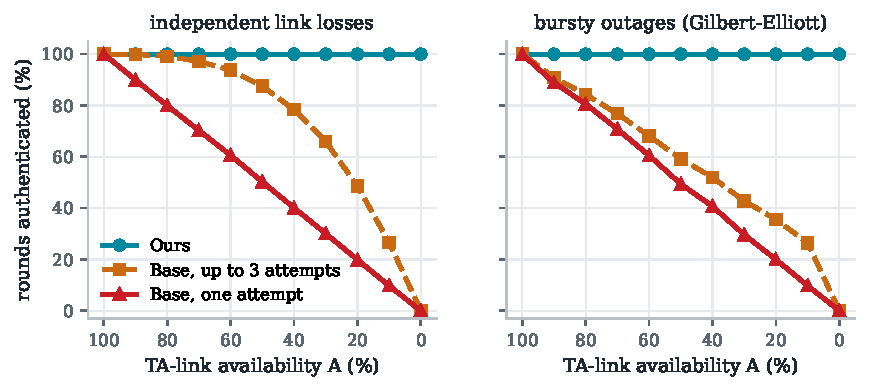
\includegraphics[width=\linewidth]{f1_availability}
\caption{Share of authentication rounds that succeed as TA-link availability falls (20\,000 rounds per point), for independent losses and for bursty
outages (Gilbert--Elliott, mean outage 10 rounds).}
\label{fig:e1}
\end{figure}
The base scheme succeeds in a round only if the satellite link is up. With $A=50\%$ it succeeds in \RAvailIidHalfOne\% of rounds, and \RAvailIidHalfThree\% if
it may retry three times, at three round-trip times. Under bursty outages, which are typical of congestion or jamming, retries help much less
(\RAvailBurstHalfThree\%) because consecutive attempts fail together. At $A=0$ the base scheme admits nobody. Ours does not use the link, so it stays at
100\% by construction (Proposition~\ref{prop:indep}). This experiment illustrates the dependency rather than discovering it.

\section{E2: time to authenticate and key a swarm}
\begin{figure}[H]
\centering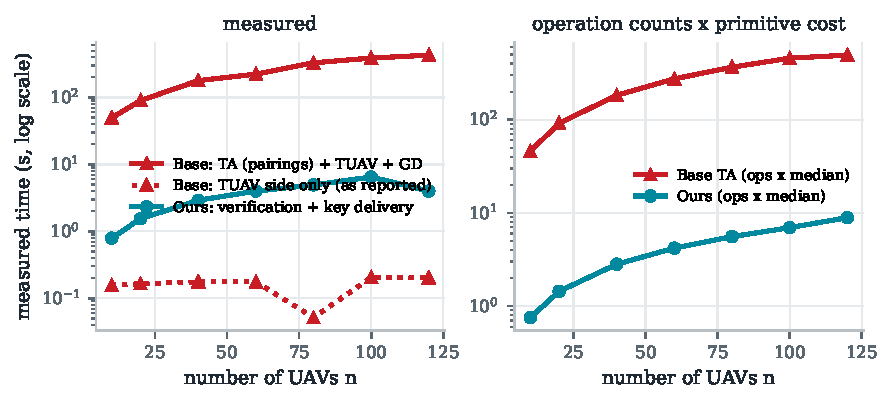
\includegraphics[width=\linewidth]{f2_latency}
\caption{Left: measured time for the TUAV to authenticate and key $n$ UAVs (ours) against the base scheme's GA1--GD4 with the TA's work included, and the
TUAV-only part the base paper reports. Right: load-independent estimate from operation counts. Log scale; satellite RTT not added. The measured $n=120$
point ran across a change in machine speed (see text).}
\label{fig:e2}
\end{figure}
\begin{table}[H]
\centering\small
\caption{E2 measurements (ms). Our time includes verification \emph{and} key delivery. The base scheme's time is split into TA (GA2), TUAV (GA3) and key distribution (GD).}
\label{tab:e2}
\pgfplotstabletypeset[col sep=comma,
  columns={n,ours_verify_ms,ours_keys_ms,ours_total_ms,base_TA_ms,base_TUAV_ms,base_GD_ms,base_total_ms,base_pairings},
  columns/n/.style={column name=$n$},
  columns/ours_verify_ms/.style={column name=Ours verify,fixed,precision=0},
  columns/ours_keys_ms/.style={column name=Ours keys,fixed,precision=0},
  columns/ours_total_ms/.style={column name=\textbf{Ours total},fixed,precision=0},
  columns/base_TA_ms/.style={column name=Base TA,fixed,precision=0},
  columns/base_TUAV_ms/.style={column name=Base TUAV,fixed,precision=0},
  columns/base_GD_ms/.style={column name=Base GD,fixed,precision=0},
  columns/base_total_ms/.style={column name=\textbf{Base total},fixed,precision=0},
  columns/base_pairings/.style={column name=Pairings},
  every head row/.style={before row=\toprule,after row=\midrule},every last row/.style={after row=\bottomrule}]{../results/e2_latency.csv}
\end{table}
For $n=\RNmax$ our TUAV authenticates and keys the swarm in \ROursTotalS\,s (\RPerUavOursMs\,ms per UAV). The base scheme needs \RBaseTotalS\,s, of which the TA's
pairings take \RBaseTaS\,s (\RPerUavBaseS\,s per UAV), before any satellite delay. Across all swarm sizes the base scheme does
\textbf{\RCountRatioLo--\RCountRatioHi$\times$ more work} by operation count (median \RSpeedup$\times$). The measured ratios for $n\le 100$ lie in the same band
(\RMeasRatioLo--\RMeasRatioHi$\times$). The $n=120$ point was re-measured while the machine changed speed between the two schemes. Its measured ratio
(\ROutlierRatio$\times$) is therefore not used; its operation-count ratio is in the band. The TUAV-only part that the base paper
reports is just \RBaseTuavShare\% of the base scheme's real work. This confirms Finding~\ref{f:cost} by measurement: the offload does not remove the cost,
it relocates it to the TA, behind the fragile link.

\section{E3: batch poisoning}
\begin{figure}[H]
\centering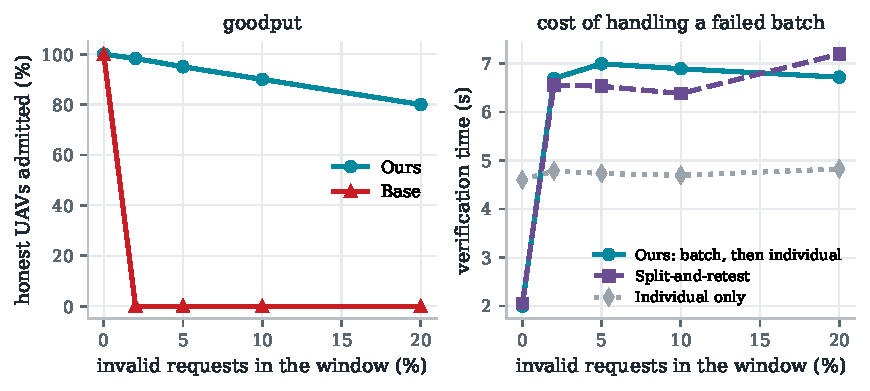
\includegraphics[width=\linewidth]{f3_poisoning}
\caption{Left: share of honest UAVs admitted as the share of invalid requests grows ($n=\RPoisonN$). Right: verification time of three strategies for handling a failed batch.}
\label{fig:e3}
\end{figure}
In the base scheme a single invalid request makes the whole batch fail, and nobody is admitted (verified for $n=10$ and in E7). With our rule every honest UAV is
admitted at every attack rate (\RPoisonGoodTwenty\% goodput when 20\% of requests are invalid, i.e.\ all honest ones). The cost is bounded as Proposition~\ref{prop:dos}
predicts: a clean window takes \RPoisonClean\,s, and the worst window (batch fails, then each request is checked) \RPoisonWorst\,s. After one failure the TUAV switches
to individual mode, whose cost is independent of the attack rate. Split-and-retest offers no advantage here, which confirms the analytical finding of
Section~\ref{sec:fallback}: with a pairing-free scheme, a batch is only a few times cheaper per signature, so re-testing halves does not pay.

\section{E4: communication}
\begin{figure}[H]
\centering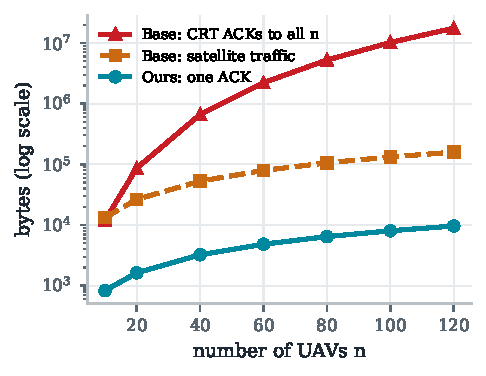
\includegraphics[width=0.62\linewidth]{f4_bytes}
\caption{Group-key traffic and the base scheme's satellite traffic, measured from the encodings of our implementation (compressed points, 32-byte hashes).}
\label{fig:e4}
\end{figure}
For $n=120$ the base scheme's acknowledgements carry \RBytesBaseKey\,MB of CRT coefficients in total. Ours sends one acknowledgement of \RBytesOursKey\,KB,
\RBytesRatio$\times$ less. The base scheme also moves \RBytesBaseSat\,KB over the satellite link for one authentication round, against zero for ours. Our join request
is larger (\RReqOurs\,B against \RReqBase\,B) because it carries the public-key material and an ephemeral value; Chapter~\ref{ch:conclusion} lists this as a limitation.

\section{E5: the vehicle tier}
\begin{figure}[H]
\centering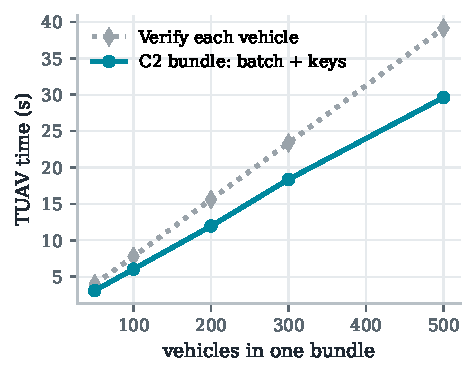
\includegraphics[width=0.62\linewidth]{f5_vehicles}
\caption{TUAV time to admit a bundle of vehicles relayed by one UAV (batch verification \emph{and} key delivery) against verifying the same requests one by one.}
\label{fig:e5}
\end{figure}
A bundle of \RVehN\ vehicles is admitted, \emph{including} key derivation and encryption, in \RVehBatchS\,s. Verifying the same requests one by one, without keys, takes
\RVehIndS\,s. A bundle from a non-member relay is dropped after one MAC check in at most \RVehDropUs\,$\mu$s, regardless of its size, so floods of forged vehicle requests
never reach signature verification.

\section{E6: handover}
\begin{figure}[H]
\centering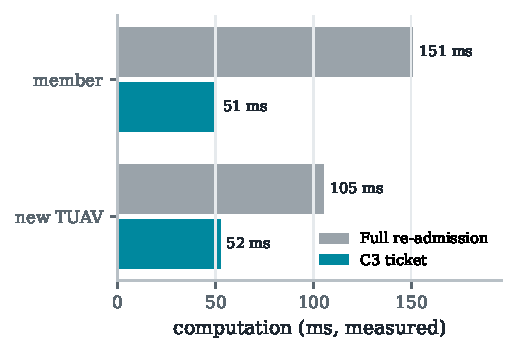
\includegraphics[width=0.62\linewidth]{f6_handover}
\caption{Computation for one handover: full re-admission in the new cell against a C3 ticket (median of 25 runs).}
\label{fig:e6}
\end{figure}
A ticket handover costs the new TUAV \RHoTuavTicket\,ms instead of \RHoTuavFull\,ms, and the member \RHoMemTicket\,ms instead of \RHoMemFull\,ms. In a one-hour mobility run
(3 cells of 2\,km, 30 UAVs at 10--20\,m/s) there were \RHoCross\ cell crossings. With a 1\,s beacon period the mean service gap per crossing falls from \RHoGapFull\,ms (wait for
the next beacon, then full admission) to \RHoGapTicket\,ms. The TUAVs' total admission CPU falls from \RHoCpuFull\,s to \RHoCpuTicket\,s.

\section{E7: attacks, executed}
\begin{table}[H]
\centering\small
\caption{Attack outcomes, executed against both implementations.}
\label{tab:e7}
\begin{tabular}{@{}lcc@{}}
\toprule
Attack & Base scheme & Ours\\
\midrule
TA forges a request for a registered UAV & \no\ succeeds & \yes\ fails\\
Two cancelling errors pass the batch check & \no\ succeeds & \yes\ fails\\
Revoked UAV recovers the new group key & \no\ succeeds & \yes\ fails\\
One invalid request blocks all honest UAVs & \no\ yes & \yes\ no\\
Old request replayed under a new beacon & -- & \yes\ rejected\\
Replayed handover ticket & -- & \yes\ rejected (test)\\
Bundle from a non-member relay & -- & \yes\ dropped (E5)\\
\bottomrule
\end{tabular}
\end{table}

\section{Summary}
Every measurement points the same way as the analysis. The base scheme's apparent efficiency comes from not counting the TA. Its key traffic grows as $n^3$.
Its batch has no failure path. Ours removes the TA from the field, is faster in total, is linear in traffic, degrades gracefully under poisoning, and
extends to vehicles and handover at modest cost.
